\subsection{Tools for Model-Driven Development}

This section will describe the most relevant tools when doing \acrfull{mdd} in the \acrlong{emf} ecosystem.

\subsubsection{Eclipse Modeling Framework and Ecore}

% What is Ecore
\paragraph*{What it is}
The \acrfull{emf} project provides tools for modeling and code generation.
\Acrshort{emf} consists of three main parts: an \emph{EMF core}, \emph{EMF.edit} and \emph{EMF.codegen}.
The core has a \gls{metamodel}, \emph{Ecore}, and a java runtime with support for change notifications, reflective \gls{API} and mechanisms for serializing to the XMI format. EMF.edit contains components for creating model editors, like labels providers and a command framework for undo/redo.
The EMF.codegen has code generation facilities which are controlled through a \texttt{genmodel} file.\cite{gronbackEclipseModelingProject}

% When? Who? Why?
\paragraph*{Using it} The framework is provided as plugins to the \gls{Eclipse}.
The modeler and user needs to have java installed, and it runs as a desktop application.

% The Ecore model
\paragraph*{The Ecore metamodel}
\Gls{Ecore} is the \gls{metamodel} used in the \acrlong{emf}.
It is an object oriented model, with concepts like \emph{EClass} and \emph{EAttribute}.
The \gls{metamodel} for Ecore is also Ecore, which means it is defined using itself.\footnote{The Ecore metamodel is available at \href{https://git.eclipse.org/c/emf/org.eclipse.emf.git/tree/plugins/org.eclipse.emf.ecore/model/Ecore.ecore}{https://git.eclipse.org/c/emf/org.eclipse.emf.git/tree/plugins /org.eclipse.emf.ecore/model/Ecore.ecore}.}

% Ecore and standards
% MOF
\paragraph*{Ecore and standards}
\Gls{Ecore} is close to the \acrfull{EMOF} specification\footnote{\href{https://www.omg.org/spec/MOF/2.4.1/PDF}{https://www.omg.org/spec/MOF/2.4.1/PDF}}, but is based on MOF Core v1.\footnote{Ecore implemented MOF, but excluded what it deemed nonessential.
Then MOF was inspired by Ecore and split into \acrshort{EMOF} and CMOF.~\cite{merksMerksMeanderingsEMF2007} They influenced each other. 
Ecore was an implementation of \acrshort{EMOF} before \acrshort{EMOF} existed.}
The \acrshort{EMOF} specification is created by \acrfull{OMG}.
The result is that \gls{Ecore} is an implementation of \gls{UML} Class Diagrams and compatible with other models based on MOF.

% XMI
\paragraph*{Serialization and XMI} When an \gls{Ecore} model is written as a text file, it needs \textit{serialization}.
The official format for serializing Ecore is \acrfull{XMI}.
\Acrshort{XMI} is based on XML, and is another standard from \acrshort{OMG}.
Models created in \gls{Ecore} can also be serialized to \acrshort{XMI}, as can their model instances.

% Genmodel
\paragraph*{Code generation with genmodel}
The genmodel is a model which augments an existing \gls{Ecore} model.
The serialization format is \acrshort{XMI}.
Ecore and the genmodel are both created with java code in mind: Ecore maps close to java concepts and datatypes, the genmodel has options for java code generation.
The genmodel can also specify which model-to-text generation templates to use.
By default it will create an \gls{Eclipse} plugin, but the target platform can also be \acrfull{RCP}\footnote{This is like the \acrshort{IDE}, but without other bundles/plugins.}, \acrfull{RAP}\footnote{A JFace renderer for the web} or \acrfull{GWT}.

% Edit and Editor?

\subsubsection{Sirius}\label{sec:sirius}
% What is Sirius?
\paragraph*{What it is} Eclipse Sirius is a framework for creating  domain-specific modeling workbenches.~\cite{eclipsefoundationSiriusEasiestWay}
It is an \gls{Eclipse} plugin, which focuses on creating visual editors like interactive diagrams.
An illustration of Sirius' internal architecture is shown in \cref{fig:sirius-architecture}.

Sirius can create editors for an existing \gls{Ecore} model, but does not rely on code generation.~\cite{eclipsefoundationSiriusEasiestWay}
The specification for the workbench is stored in a \texttt{.odesign} file.
A workbench can have multiple representations of a model, and the representations are stored in a \texttt{.aird} file.
Both of these files are \acrshort{XMI} serializations.

\begin{figure}[htbp]  % order of priority: h here, t top, b bottom, p page
  \centering
  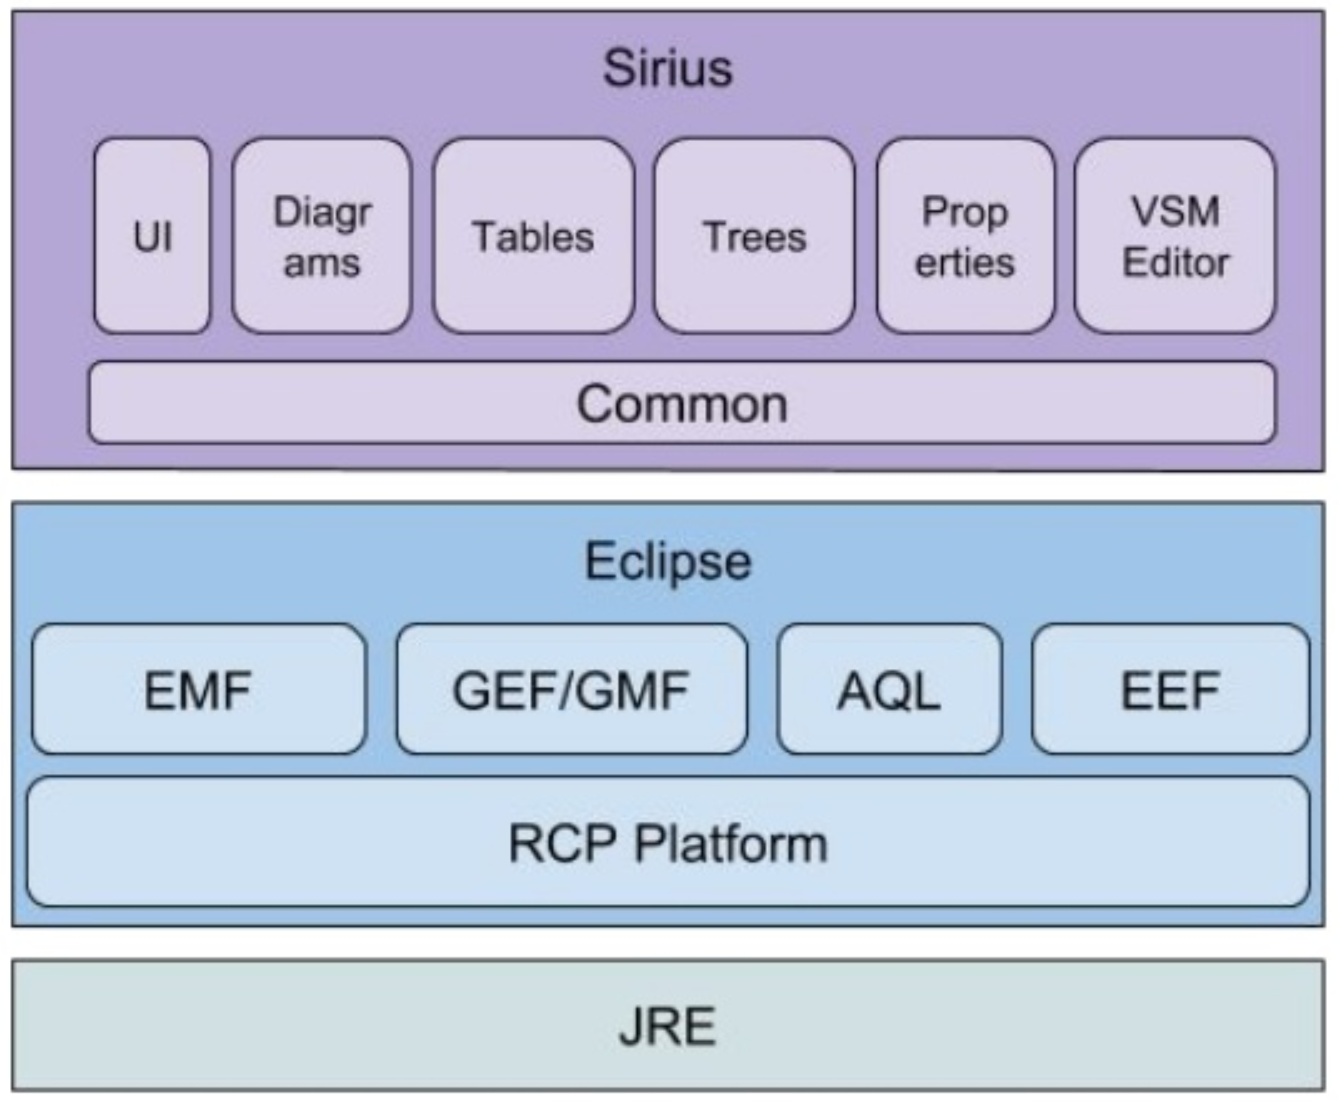
\includegraphics[width=\textwidth]{figures/Sirius_architecture}
  \caption[The Sirius Architecture]{The diagram shows the different components in Eclipse Sirius. The components on the top depend on the components below.~\cite[p.~36]{davidSiriusCon2018Sirius2018}.}\label{fig:sirius-architecture}
\end{figure}

\paragraph*{Using it} A developer creates Sirius specifications using the \gls{Eclipse}.
After a workbench is designed, the developer produces an Eclipse \emph{plugin} to distribute the graphical modeling tool. An end-user which edits model instances would install the plugin into their \gls{Eclipse}.

% When? Who? Why?

\subsubsection{Sirius Web}
%TODO: Write
% What is Sirius Web?
% When? Who? Why?

\paragraph*{What it is}
Sirius Web is an ongoing effort\footnote{As of 2020. It is supposed to be ready near the start of 2021.} to move the end-user editors of Sirius to the web.
The goal is to allow end-users to model with their browsers, instead of the \gls{Eclipse}.
Sirius Web will be \gls{open source}.
An illustration of Sirius Web's internal architecture is shown in \cref{fig:sirius-web-architecture}. Note that this is a work in progress, so the actual architecture may deviate once Sirius Web is released.
The end-user will only see the \emph{Sirius Web Frontend} (or \emph{Sirius \acrshort{RCP}}, which is the old Sirius in \cref{sec:sirius}).

Sirius Web does not use Theia, but its representations \textit{can} be shown in Theia.~\cite{neilmackenzieSiriusWebXText2020}

\paragraph*{Using it} A developer creates Sirius specifications in \emph{Eclipse Sirius} or \emph{Obeo Designer} as before. 
Then they deploy the specifications as a Sirius Web editor, instead of an Eclipse plugin.

\begin{figure}[htbp]  % order of priority: h here, t top, b bottom, p page
  \centering
  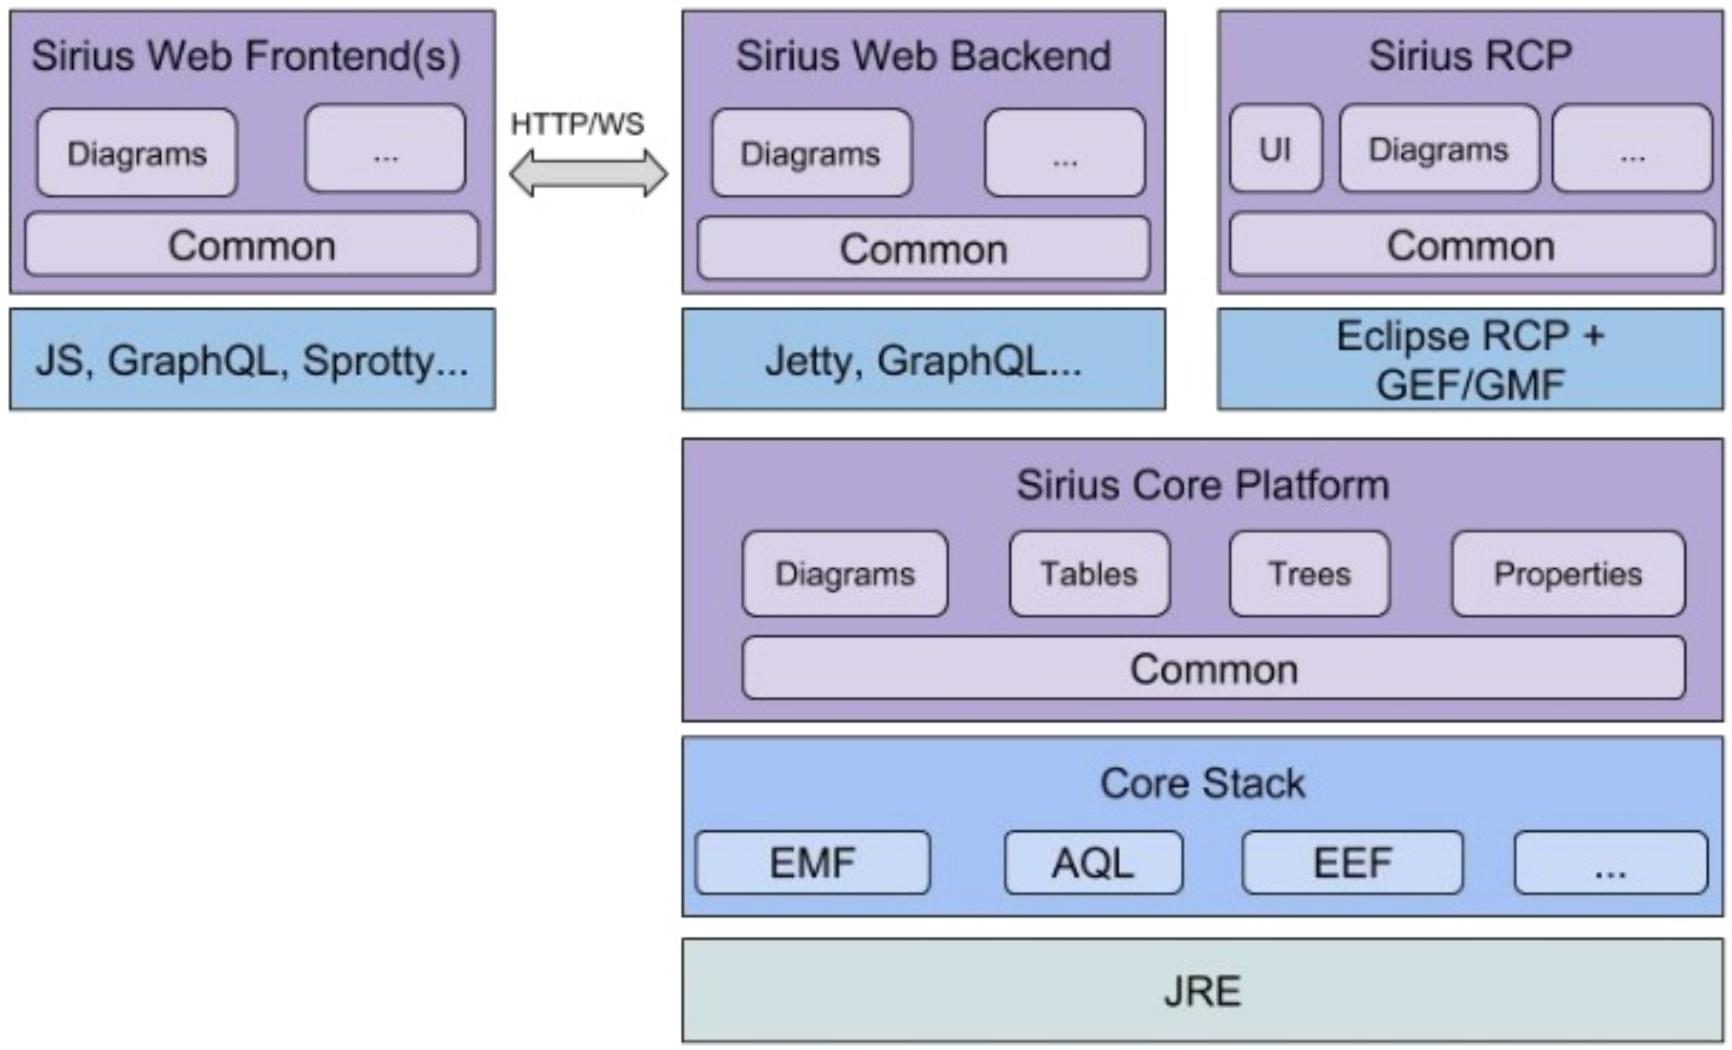
\includegraphics[width=\textwidth]{figures/Sirius-future-web-architecture}
  \caption[The Sirius Web Architecture]{The diagram shows the different components that will be in Sirius Web. Components on the top depend on components below.~\cite[p.~37]{davidSiriusCon2018Sirius2018}}\label{fig:sirius-web-architecture}
\end{figure}
